% for section-numbered lemmas etc., use "numberwithinsect"
\documentclass[a4paper,english,numberwithinsect]{eurocg18}

% the recommended bibstyle
\bibliographystyle{plainurl}

%------------------------------------------------------------------- 
%if unwanted, comment out or use option "draft"
\usepackage{todonotes}
\usepackage{microtype}
\usepackage[noend, linesnumbered]{algorithm2e}
\usepackage{amsmath}
\usepackage{color}
\usepackage{cite}
\usepackage{pifont}
\usepackage{enumerate}
\usepackage[basic]{complexity}
\usepackage{subcaption}
\usepackage{wrapfig}
\usepackage{graphicx}

% Line numbers are helpful for refereeing
\usepackage[mathlines]{lineno}
\newcommand*\patchAmsMathEnvironmentForLineno[1]{%
\expandafter\let\csname old#1\expandafter\endcsname\csname #1\endcsname
\expandafter\let\csname oldend#1\expandafter\endcsname\csname end#1\endcsname
\renewenvironment{#1}%
     {\linenomath\csname old#1\endcsname}%
     {\csname oldend#1\endcsname\endlinenomath}}%
\newcommand*\patchBothAmsMathEnvironmentsForLineno[1]{%
  \patchAmsMathEnvironmentForLineno{#1}%
  \patchAmsMathEnvironmentForLineno{#1*}}%
\AtBeginDocument{%
\patchBothAmsMathEnvironmentsForLineno{equation}%
\patchBothAmsMathEnvironmentsForLineno{align}%
\patchBothAmsMathEnvironmentsForLineno{flalign}%
\patchBothAmsMathEnvironmentsForLineno{alignat}%
\patchBothAmsMathEnvironmentsForLineno{gather}%
\patchBothAmsMathEnvironmentsForLineno{multline}%
}
\linenumbers

%helpful if your graphic files are in another directory
%\graphicspath{{./graphics/}}

% Author macros::begin %%%%%%%%%%%%%%%%%%%%%%%%%%%%%%%%%%%%%%%%%%%%%%%%
%\newcommand\polylog{{\rm polylog}}

% Author metadata::begin %%%%%%%%%%%%%%%%%%%%%%%%%%%%%%%%%%%%%%%%%%%%%%%%
\title{Maximizing Ink in Symmetric Partial Edge Drawings of $k$-plane Graphs}
%{Maximal Symmetric Partial Edge Drawings With Degree $ > 2$}
%optional, in case that the title is too long; 
%the running title should fit into the top page column
%\titlerunning{MaxSPEDs with degree $ > 2$}

%% Please provide for each author the \author and \affil macro, 
%even when authors have the same affiliation, i.e. for each 
%author there needs to be the  \author and \affil macros
\author[1]{Michael H\"oller}
\author[1]{Fabian Klute}
\author[1]{Soeren Nickel}
\author[1]{Martin~N\"ollenburg}
\author[1]{Birgit Schreiber}

\affil[1]{Algorithms and Complexity Group, TU Wien, Vienna, Austria\\ \texttt{[fklute|noellenburg]@ac.tuwien.ac.at}}
%\affil[2]{Algorithms and Complexity Group, TU Wien, Vienna, Austria} %\texttt{fklute@ac.tuwien.ac.at}}
%\affil[3]{Algorithms and Complexity Group, TU Wien, Vienna, Austria \texttt{}}
%\affil[4]{Algorithms and Complexity Group, TU Wien, Vienna, Austria} %\texttt{noellenburg@ac.tuwien.ac.at}}
%\affil[5]{Algorithms and Complexity Group, TU Wien, Vienna, Austria \texttt{}}
%mandatory. First: Use abbreviated first/middle names. 
%Second (only in severe cases): Use first author plus 'et. al.'
\authorrunning{M. Höller, F. Klute, S. Nickel, M. N\"ollenburg, and B. Schreiber} 

% Author macros::end %%%%%%%%%%%%%%%%%%%%%%%%%%%%%%%%%%%%%%%%%%%%%%%%%

\newcommand{\martin}[1]{\todo[inline,color=blue!40]{MN: #1}}
\newcommand{\fabian}[1]{\todo[inline,color=pink!40]{FK: #1}}
\newcommand{\birgit}[1]{\todo[inline,color=red!40]{BS: #1}}
\newcommand{\michael}[1]{\todo[inline,color=green!40]{MH: #1}}
\newcommand{\soeren}[1]{\todo[inline,color=orange!40]{SN: #1}}

\newcommand{\ped}{\ensuremath{\textsc{PED}}\xspace}
\newcommand{\maxsped}{\ensuremath{\textsc{MaxSPED}}\xspace}
\newcommand{\ppsat}{\ensuremath{\textsc{Planar 3-Sat}}\xspace}
\newcommand{\sollong}{\ensuremath{\textit{long}}\xspace}
\newcommand{\solmid}{\ensuremath{\textit{mid}}\xspace}
\newcommand{\solshort}{\ensuremath{\textit{short}}\xspace}

\begin{document}

\maketitle

\begin{abstract}
	Partial edge drawing (PED) is a drawing style for non-planar graphs, in which edges are drawn only partially as pairs of opposing stubs on the respective end-vertices. 
	In a PED, by erasing the central parts of edges, all edge crossings and the resulting visual clutter are hidden in the undrawn parts of the edges.
	We study symmetric partial edge drawings (SPEDs), in which the two stubs of each edge are required to have the same length. 
	It is known that maximizing the ink (or the total stub length) when transforming a straight-line drawing with crossings into a SPED is tractable for 2-plane input drawings, but generally \NP-hard.
	We show that the problem remains \NP-hard even for 3-plane input drawings.
	Yet, for $k$-plane input drawings whose edge intersection graph forms a collection of trees or cacti we present efficient algorithms for ink maximization.
\end{abstract}

\section{Introduction}

Visualizing non-planar graphs as node-link diagrams is challenging due to the visual clutter caused by edge crossings. The layout readability deteriorates as the edge density and thus the number of crossings increases.
Therefore alternative layout styles are necessary for non-planar graphs.
A radical approach first used in applied network visualization work by Becker et al.~\cite{bew-vnd-95} is to start with a traditional straight-line graph drawing and simply drop a large central part of each edge and with it many of the edge crossings.
This idea relies on the closure and continuation principles in Gestalt theory, which imply that humans can still see a full line segment based only on the remaining edge stubs by filling in the missing information in our brains.
User studies have confirmed that such drawings remain readable while reducing clutter significantly~\cite{bvkw-epdldge-12,bkl-us-15}.

\begin{wrapfigure}[11]{r}{0.45\textwidth}
	\centering
	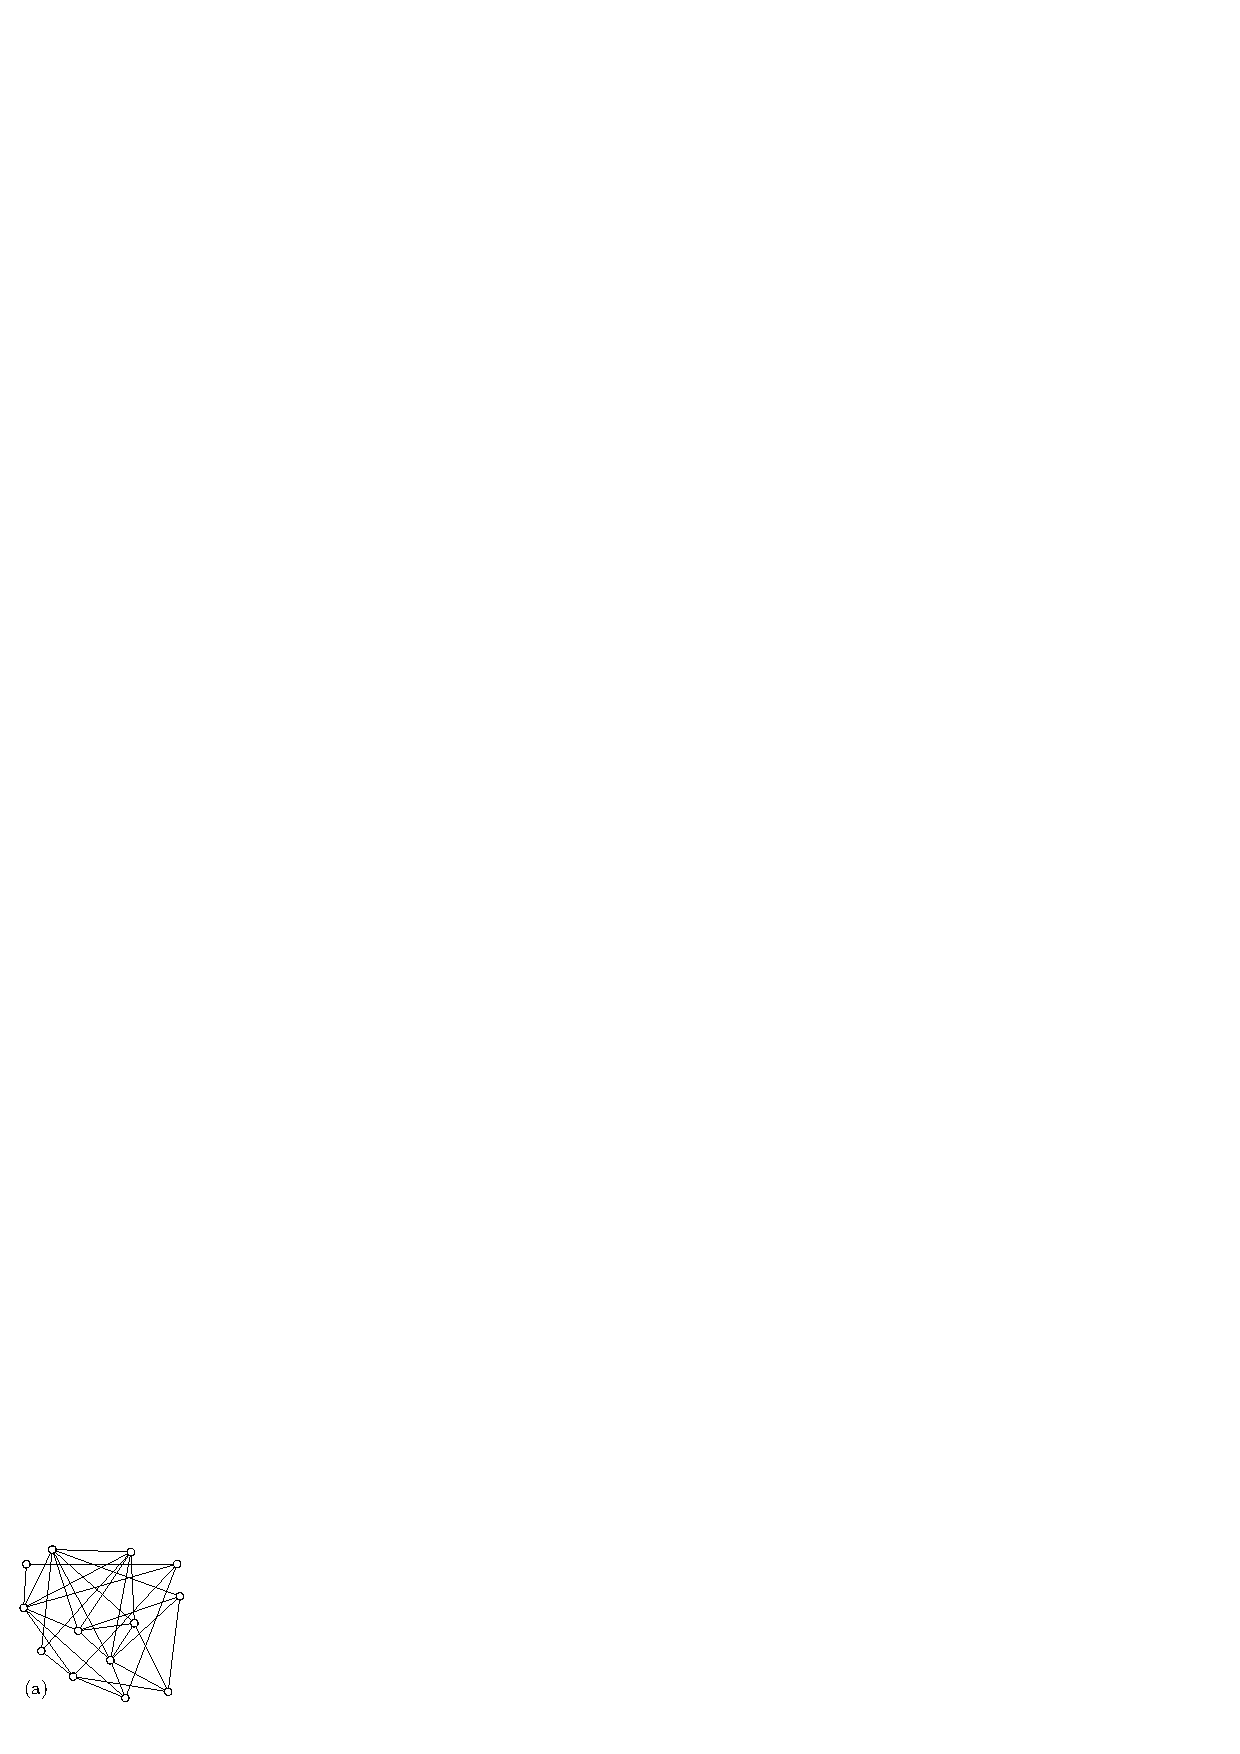
\includegraphics{export_full}
	\hfill
	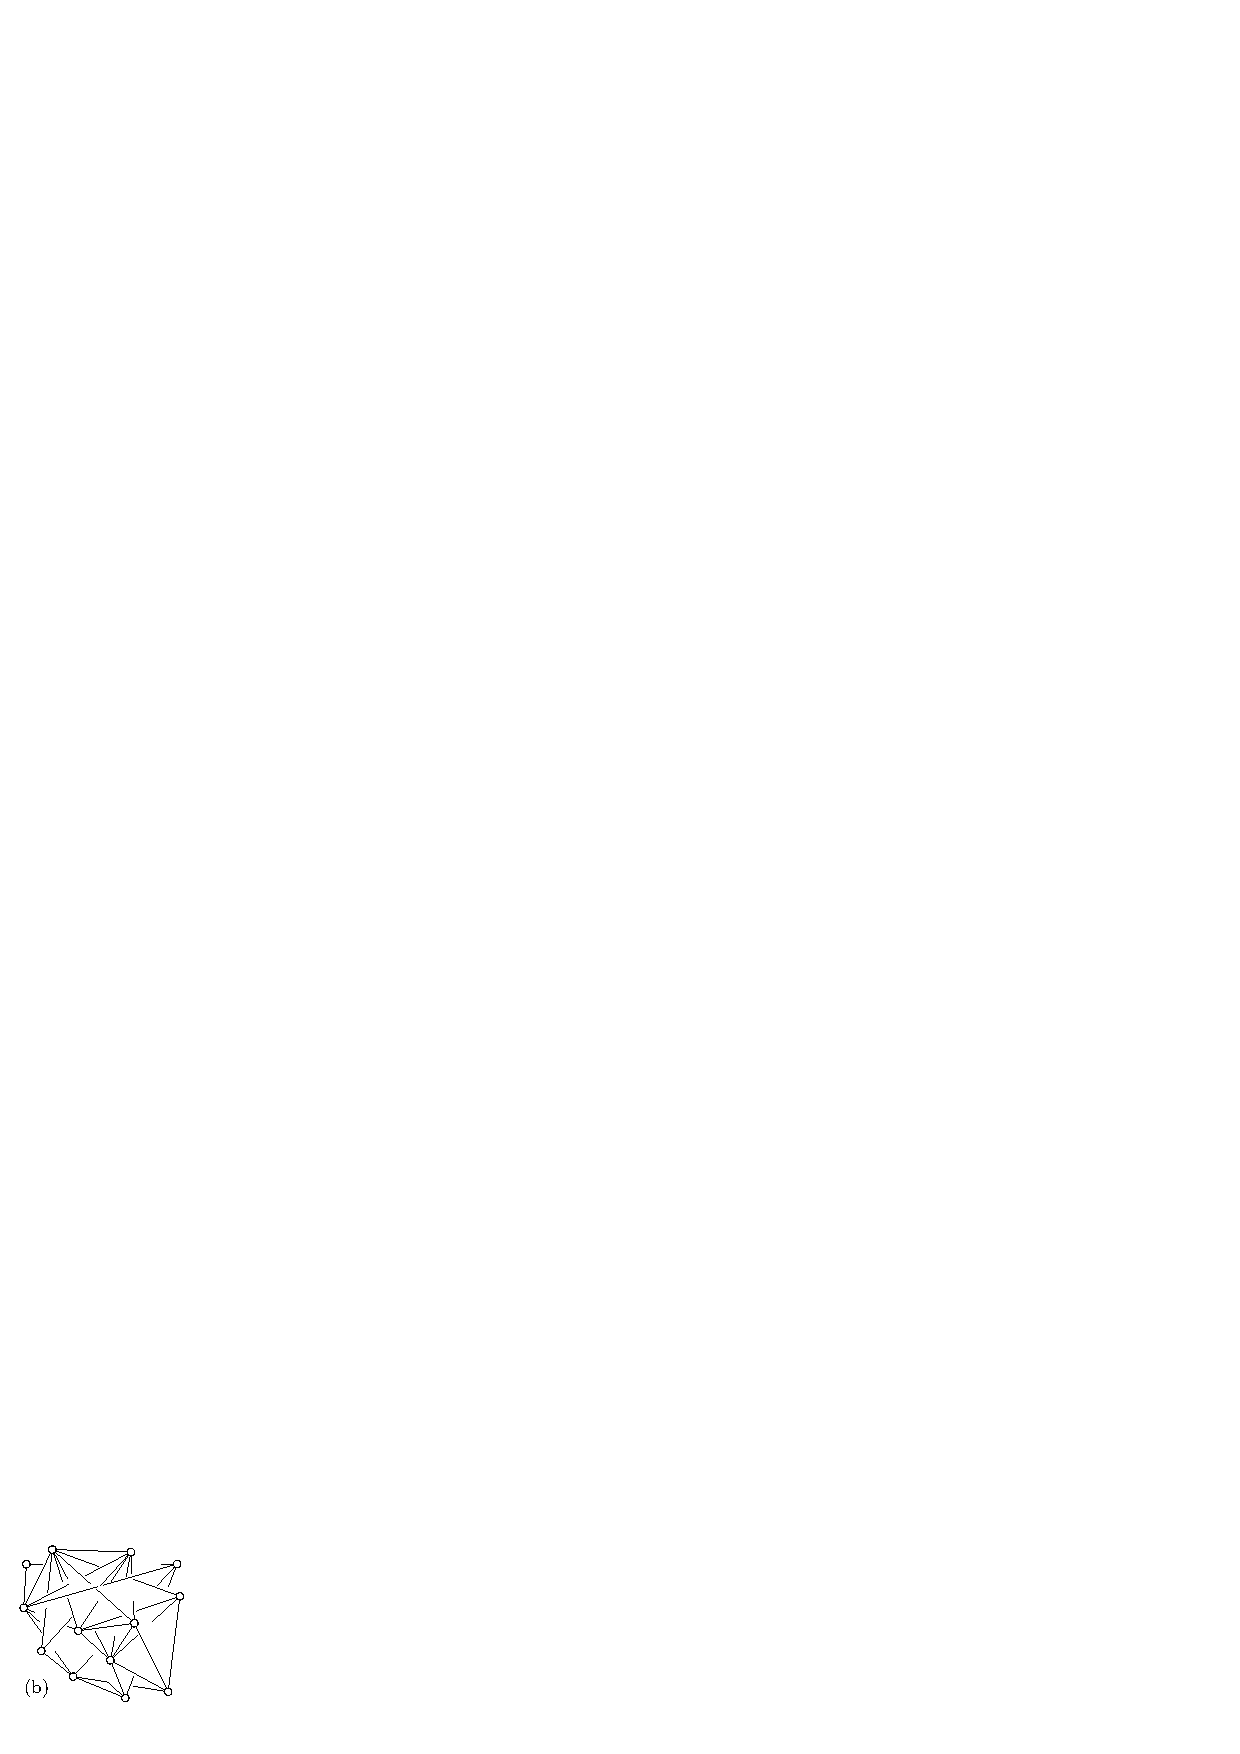
\includegraphics{export_alpha_nontouching}
	\caption{A straight-line graph drawing (a) and a maximum-ink symmetric partial edge drawing (b) of the same graph.}
	\label{fig:examples}
\end{wrapfigure}


The idea of drawing edges only partially has been formalized in graph drawing as follows~\cite{bk-ecbe-12}. 
A \emph{partial edge drawing (PED)} is a graph drawing that maps vertices to points and edges to pairs of crossing-free edge stubs of positive length pointing towards each other.
These edge stubs are obtained by erasing one contiguous central piece of the straight-line segment connecting the two endpoints of each edge.
In other words each straight-line edge is divided into three parts, of which only the two outer ones are drawn, see Fig.~\ref{fig:examples}.
More restricted and better readable~\cite{blmt-pedhmitc-16} variations of PEDs are \emph{symmetric} PEDs, in which both stubs of an edge must have the same length (see Fig.~\ref{fig:examples}(b)), and \emph{homogeneous} PEDs, in which the ratio of the stub length to the total edge length is the same for all edges.
The natural optimization problem in this formal setting is \emph{ink maximization}, i.e., maximizing the total stub length, so that as much information as possible is given in the drawing while all crossings disappear in the negative background space. 


We study the ink maximization problem for symmetric partial edge drawings (SPEDs) with a given geometric input drawing.
This problem is known as \maxsped. 
Bruckdorfer and Kaufmann~\cite{bk-ecbe-12} presented an integer linear program for solving \maxsped. 
Later, Bruckdorfer et al.~\cite{bcgkmn-pped-17} gave an $O(n \log n)$-time algorithm for \maxsped on the class of 2-plane input drawings (no edge has more than two crossings), where $n$ is the number of vertices, and an efficient 2-approximation algorithm for the dual problem of minimizing the amount of erased ink for arbitrary input drawings.
Bruckdorfer~\cite{b-sgh-15} further gives an \NP-hardness proof for \maxsped.

\medskip

\noindent\textbf{Contribution.} We extend the results of Bruckdorfer et al.~\cite{bcgkmn-pped-17} on 2-plane geometric graph drawings to $k$-plane graph drawings for $k > 2$. 
In particular, we show that \maxsped is \NP-hard even for 3-plane input drawings. 
However, for $k$-plane graph drawings whose edge intersection graphs are collections of trees or cacti (which have maximum degree $k$), we give polynomial-time algorithms for solving \maxsped.





\section{Preliminaries}\label{sec:preliminaries}
%\begin{itemize}
%	\item basic definitions and notation
%	\item segment intersection graph
%	\item alle planaren Graphen können auftreten (insbes. Bäume und Kakteen)
%\end{itemize}
%Input: $k$-plane graph drawing $\Gamma$ of a graph $G$ with edge set $S={s_1, \dots, s_m}$ (set of segments)
%Intersection graph $C=(V,E)$ with $V=S$ and edges if two segments intersect 
%Consider maximum degree of $C$ -- here mostly 3.

Throughout the paper let $ G $ be a \emph{simple graph} with edge set $ S = \{s_1,\dots,s_m\}$ and $ \Gamma $ a straight line drawing of $ G $ in the plane. We call $ \Gamma $ \emph{$ k $-plane} if every edge $ s_i \in S $ is crossed by at most $ k $ other edges from $ S $ in $ \Gamma $. We use the terms edge in $ S $ and segment in $ \Gamma $ interchangeably, since our input is always a graph $G$ with a given drawing $ \Gamma $. Hence we can also interpret $S$ as a set of line segments.

The \emph{intersection graph} $ C = (V,E) $ of $ \Gamma $ is the graph containing a vertex $v_i$ in $ V $ for every $ s_i \in S $ and an edge $ v_i v_j \in E $ between vertices $ v_i, v_j \in V $ if the corresponding edges $ s_i, s_j \in S $ intersect in $ \Gamma $. Observe that the intersection graph $ C $ of a $ k $-plane drawing $ \Gamma $ has maximum degree $ k $.  

Using a standard sweep-line algorithm, computing the intersection graph $C$ of a set of $m$ line segments takes $O(m \log m + I)$ time~\cite{bcko-cgaa-08}, where $I$ is the number of intersections, i.e., the number of edges of $C$. 

%\fabian{This part has to be adapted once the intro is fixed}
%
%We define a \emph{partial edge drawing} (\ped) $ \Gamma' $ of $ G $ as a drawing using the same embedding as $ \Gamma $, but edges are drawn as \emph{stubs}, i.e., we do not depict an edge $ s_i \in S $ by a line segment connecting the two vertices, but remove the middle part of the edges such that no two stubs intersect in $ \Gamma' $. We call a \ped $ \Gamma' $ \emph{symmetric} if for every edge $ s_i s_j \in S $ its two stubs have equal lengths in $ \Gamma' $. Finally we define the problem \maxsped as finding a symmetric \ped $ \Gamma' $ of $ G $ where the sum of the lengths of the stubs is maximized. This is also known as ink maximization~\cite{bcgkmn-pped-17}.
%
%\martin{Maybe we don't need the above paragraph as PED, SPED, maxSPED are all somewhat defined in the introduction}

\section{Hardness of \maxsped for $k\ge3$}\label{sec:hardness}
\soeren{Should the graph in this section too be called G and its drawing $\Gamma$? Also,~\cite{b-sgh-15} claims, paths need to have not only even but equal length, which seems plausible and helps my argument. I'm however not sure if it is actually necessary.}

In this section we close the gap between the known hardness of \maxsped~\cite{b-sgh-15} and the polynomial-time algorithm for 2-plane drawings~\cite{bcgkmn-pped-17} as summarized in the following theorem.

\begin{theorem}\label{thm:hard}
	The problem \maxsped is \NP-hard even for 3-plane graph drawings.
\end{theorem}

\begin{proof}
	We reduce from the \NP-hard problem \ppsat~\cite{l-pftu-82} using similar ideas as Bruckdorfer's~\cite{b-sgh-15} general proof of the hardness of \maxsped. %, which reduces from the more restricted problem \textsc{Planar Positive 1-in-3 Sat}. 
	Let $\phi$ be a planar 3-Sat formula with $n$ variables $\{x_1, \dots, x_n\}$ and $m$ clauses $\{c_1, \dots, c_m\}$, each consisting of three literals.
	We can assume that $\phi$ comes with a planar drawing of its variable-clause graph $H_\phi$ that has a vertex for each variable $x_i$ placed on a horizontal line and a vertex for each clause $c_j$ connected on one side of the horizontal line to the three variables appearing in $c_j$. 
	In our gadget-based reduction we create a 3-plane drawing $\Gamma_\phi$ as a set of line segments of uniform length and a value $L$ such that $\Gamma$ has a SPED of total ink at least $L$ if and only if $\phi$ is satisfiable.
	
	All segments are of length 5.
	We construct our gadgets using pairs of intersecting segments, one colored green, the other one red.
	Their mutual intersection point is at distance 1 from an endpoint, which has the effect that the maximum amount of ink contributed by such a pair is 7 (one full segment and the other one with two stubs of length 1 each).
	


% To show that \maxsped is \NP-hard even for 3-plane input drawings, we will provide a reduction from the \NP-hard \ppsat to \maxsped, similar to Till Bruckdorfers Dissertation \cite{b-sgh-15}. An incremental explanation of \ppsat would be: Given a formula $\phi$ in 3-CNF, in which every single occurring literal is not negated (positive). Consider the graph $P(\phi)$ that contains a vertex for each clause (clause vertex) and a vertex for each variable (variable vertex) and every variable vertex is connected via an edge with a clause vertex, if and only if the variable occurs in the corresponding clause. If $P(\phi)$ is planar, $\phi$ and a planar embedding $\Pi$ of $P(\phi)$ is an instance of \ppsat. The problem is to decide whether $\phi$ has a satisfying truth assignment, such that only one (and since it is a satisfying assignment, exactly one) variable in each clause is set to true.

\begin{figure}
	\centering
	\hfill
	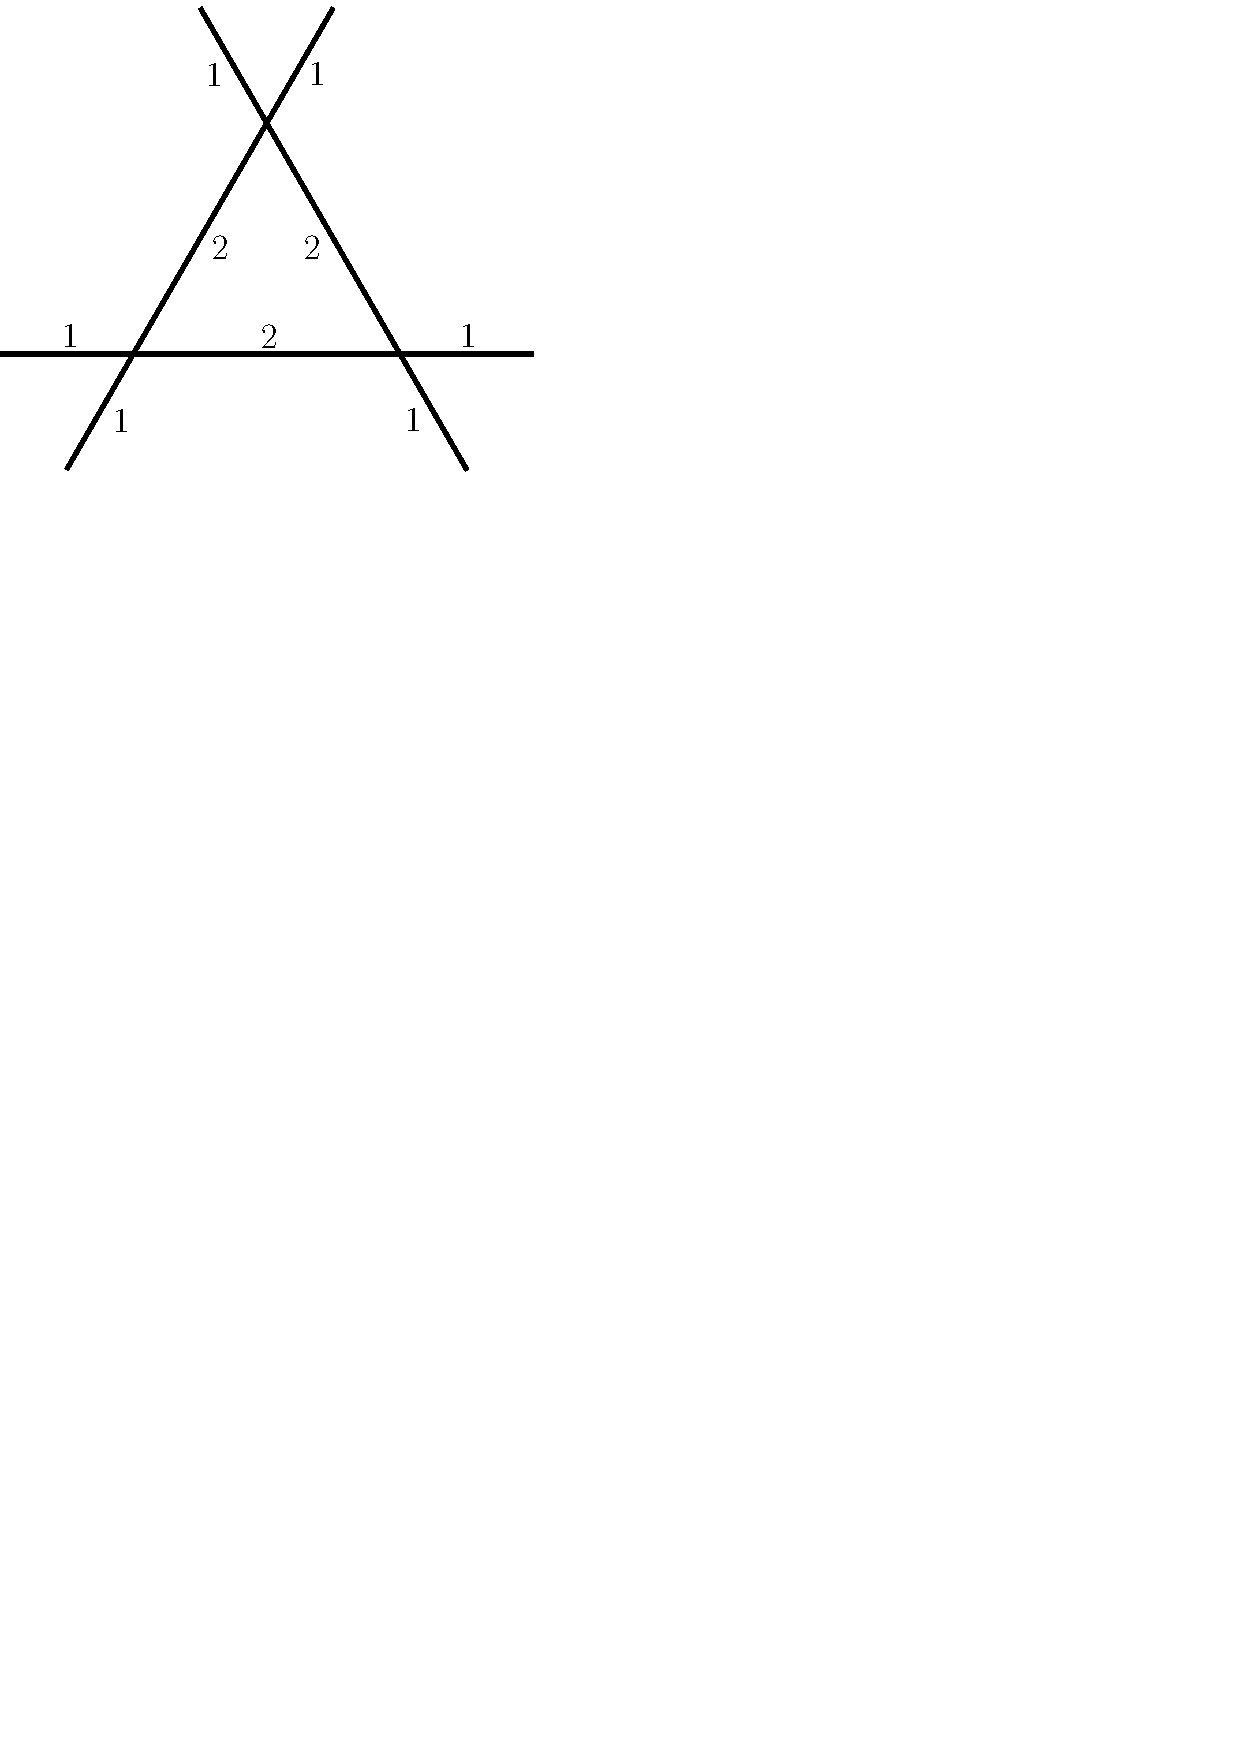
\includegraphics[width=.2\linewidth]{clause_to_triangle}
	\hfill
	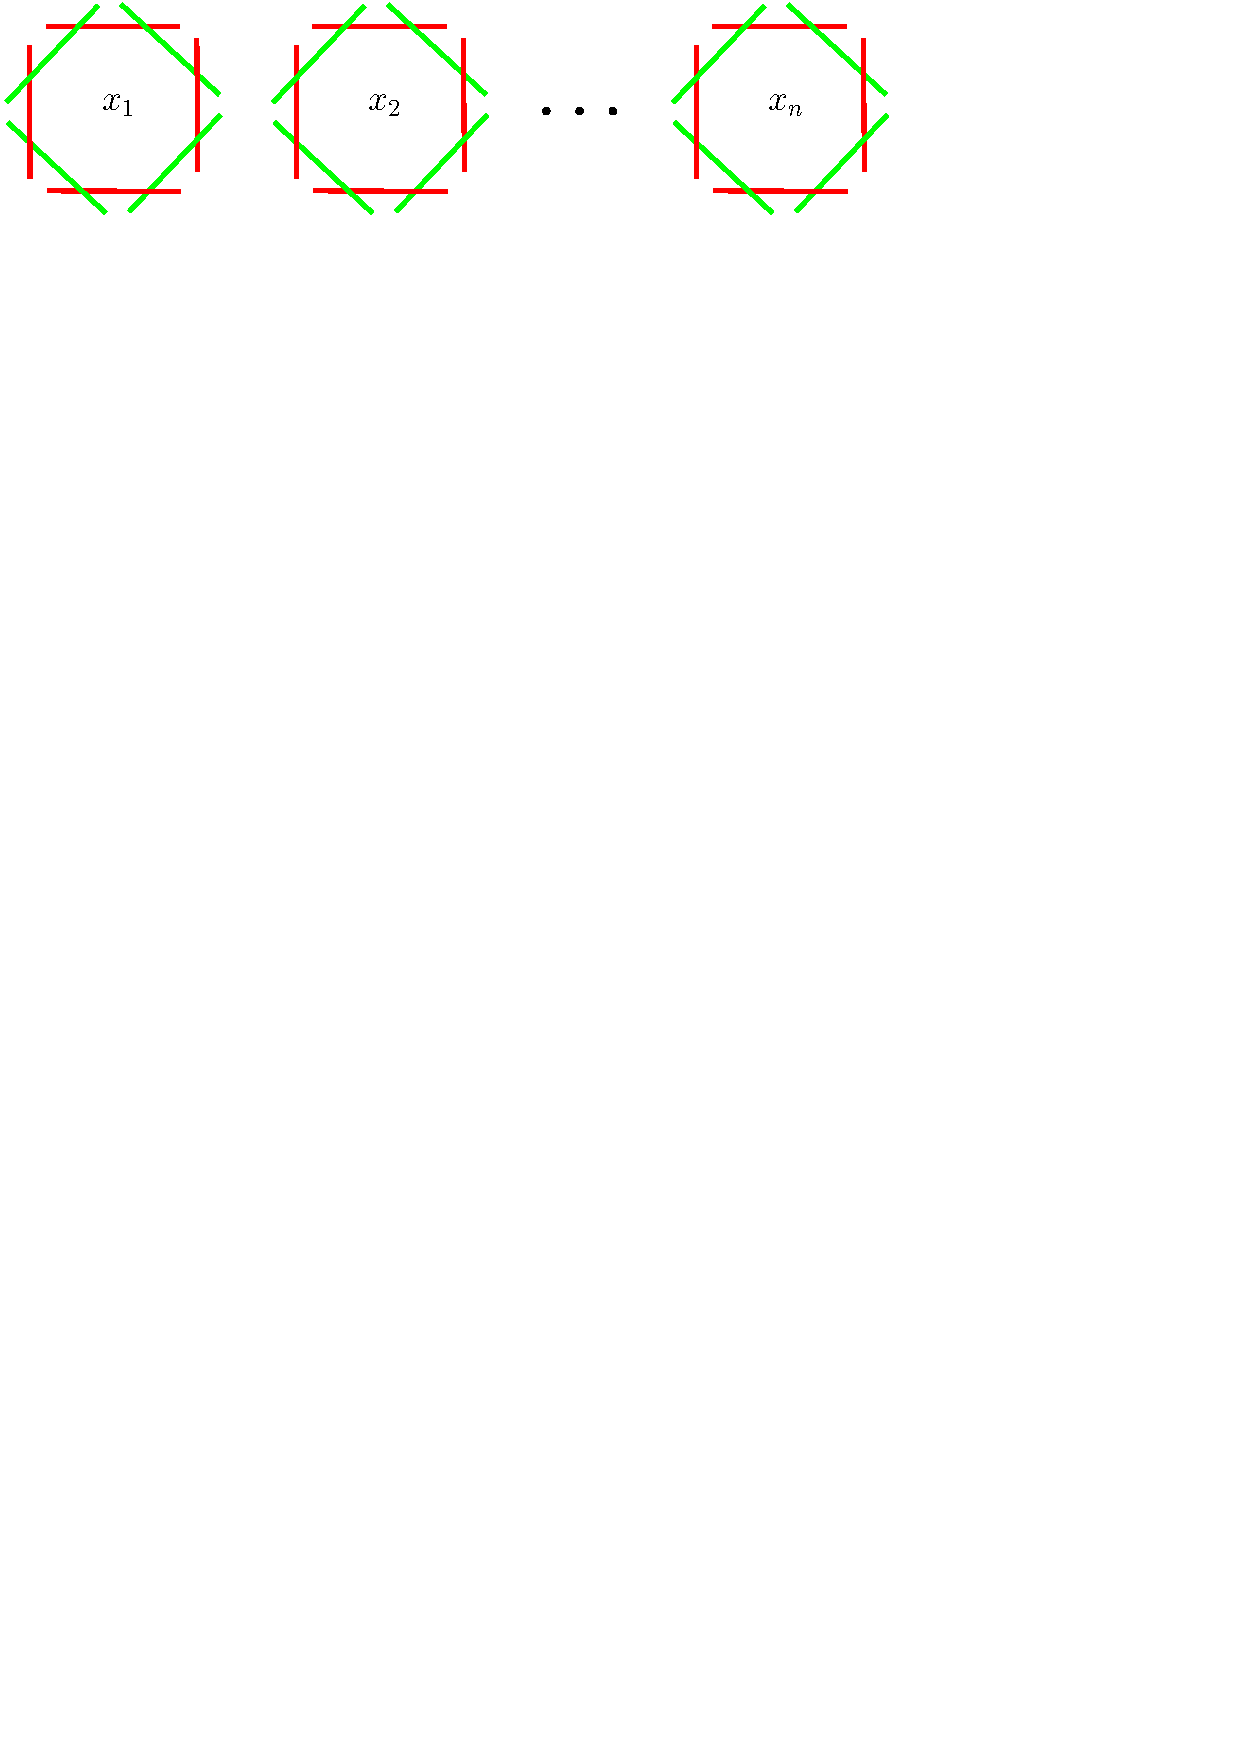
\includegraphics[width=.5\linewidth]{variable_to_circle}
	\caption{A triangle representing a clause, with unit lengths (a) and circles of segments representing variables, coloured in red and green (b).}
	\label{fig:gadgets}
\end{figure}

% We create a graph G which is an instance of \maxsped out of an instance of \ppsat by creating the following components.

%\begin{itemize}
%	\item a triangle of overlapping lines for every clause vertex (Fig.~\ref{fig:gadgets} (a))
%	\item a circle of overlapping lines of even length for every variable vertex (Fig.~\ref{fig:gadgets} (b))
%	\item a path of overlapping lines of even length for every connection between a variable vertex and a clause vertex in $\Pi$ (Fig.~\ref{fig:gadget_connection})
%\end{itemize}

A triangle (gadget clause) of overlapping lines $l_{x_a}$, $l_{x_b}$, and $l_{x_c}$ is constructed for each clause $(x_a \lor x_b \lor x_c)$ such that each edge of the trinagle is split into two stubs of length 1 and a middle part of length 2 (see Fig~\ref{fig:gadgets}(a)). Each edge of this clause gadget will be connected to exactly one variable gadget since every clause in $\phi$ consists of exactly three literals. Observe that only one edge at a time can be drawn completely since it intersects both other edges, that the optimal solution in terms of maximized ink is drawing one edge completely (4 units) and the stubs of the other two edges (2 units respectively), so 8 units in total and that all three solutions are equivalent.

\begin{wrapfigure}[11]{r}{0.45\textwidth}
	\centering
	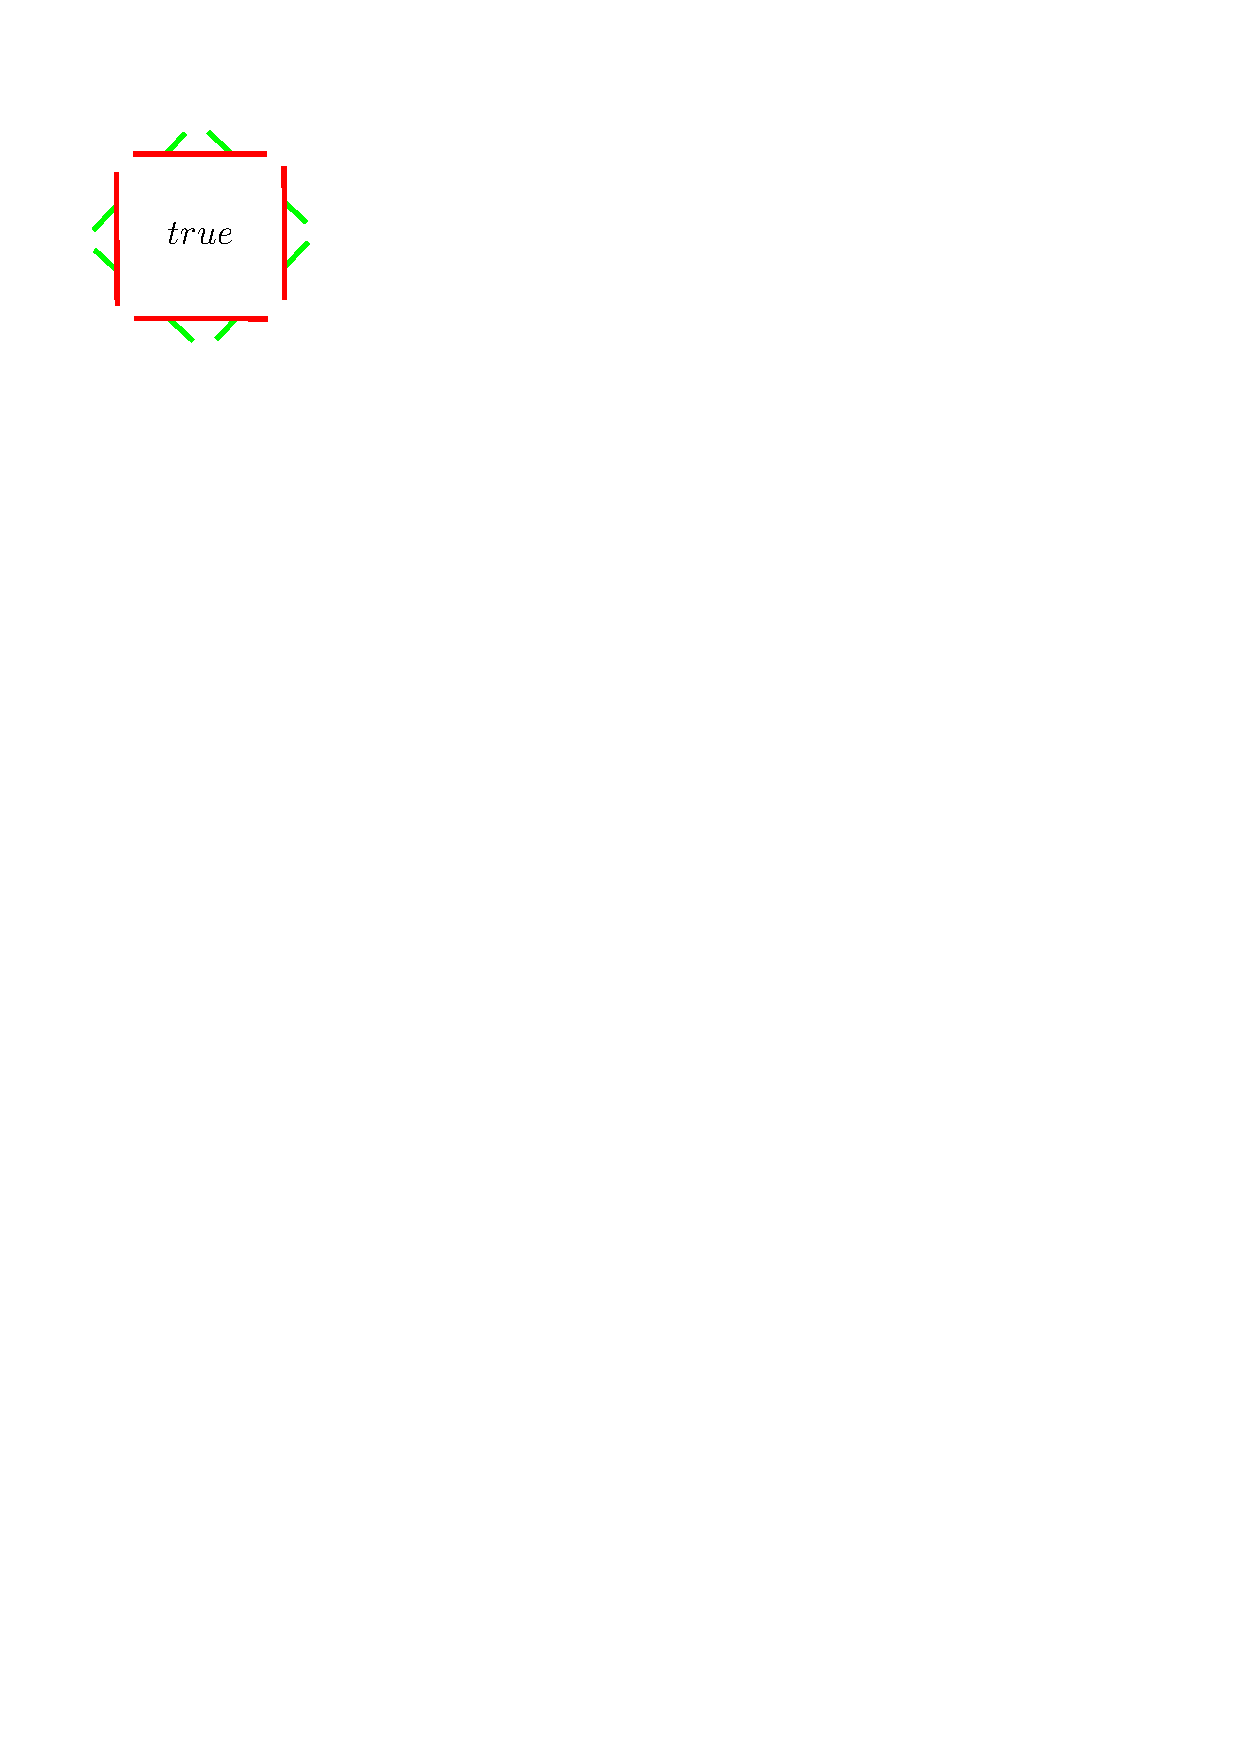
\includegraphics[width=.45\linewidth]{circle_true}
	\hfill
	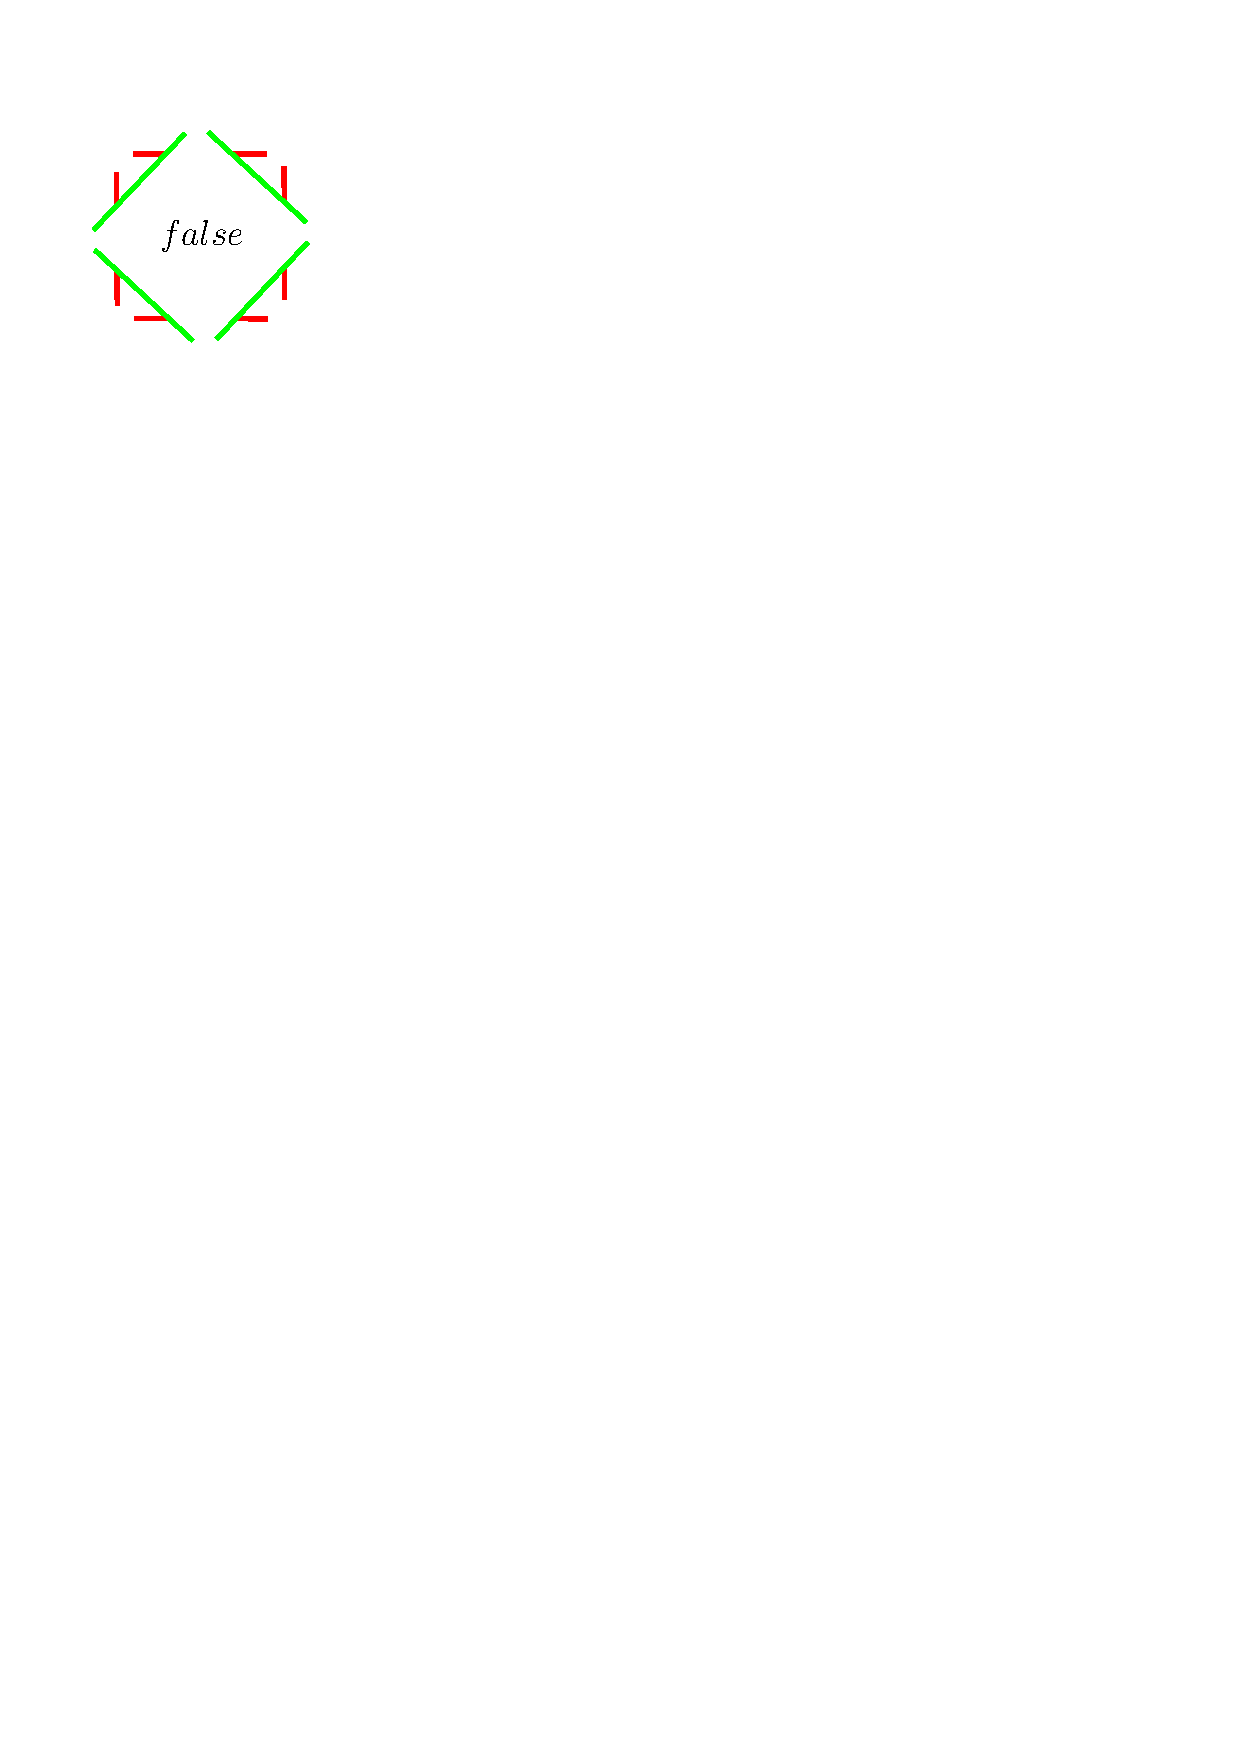
\includegraphics[width=.45\linewidth]{circle_false}
	\caption{Variable gadget representing a true variable (a) and a false variable (b)}
	\label{fig:optimal_circles}
\end{wrapfigure}

Circles of segments (variable gadgets) are constructed in a very similar fashion. Let $m$ be the maximum number of clauses in which a single variable appears. Every variable $x_n$ will be represented by $m$ pairs of segments one red and one green which are connected as seen in Fig.~\ref{fig:gadgets} (b) and form a circle. It can be observed that every segment $s_n$ intersects exactly 2 other segments $s_{n-1}$ and $s_{n+1}$ ($s_{2m}$ intersects with $s_1$ to create the circle). These intersections split every segmet in three parts, which again have length 1 for the stubs and 2 for the middle part. If $x$ is true, the green edges will be drawn completely, if it is false the red edges will be drawn completely. Observe that fixing a green edge to be drawn completely fixes all green edges to be drawn completely, like in Fig.~\ref{fig:optimal_circles} (a) (in order to have an optimal solution for this circle) and conversely for the red edges, like in Fig.~\ref{fig:optimal_circles} (b). We will associate the first version, with subdivided green edges, with the variable being true and the second one with the variable being false. Since all edges are cut in the same fashion, the two solutions are equivalent in terms of maximized ink and amount to $4m + 2m = 6m$.

The variable clauses are arranged on a spine and the clause gadgets are placed above or below the spine, according to the planar embedding of the \ppsat. Then the clause gadgets are connected to the variable gadgets corresponding to the occuring variables via segment chains (see Fig.\ref{fig:gadget_connection}, segment chains are for the sake of visualization not all equally long). These chains are composed of $t$ (where $t$ is an sufficiently large even integer) equal length segments $s_1$, \dots, $s_t$, which are again coloured alternatingly red and green. Every segment $s_i$ crosses with $s_{i-1}$ (except for $s_1$) and $s_{i+1}$ (except for $s_t$). All segments are divided again into 3 parts with the stubs having length 1, and the middle part having length 2. $s_1$ is also split in this ratio by one of the green stubs of a variable gadget, however the stub is intersected such that the remaining stub has length $1-\varepsilon$. The same holds for $s_t$ and a stub of an edge in the clause gadget. Here again the optimal solution in terms of maximizing ink is by drawing either all green edges completely and all red ones as stubs, or vice versa. Both solutions have a value of $4\frac{t}{2} + 2\frac{t}{2} = 3t$. It should be noted that completely drawing the red edges cuts of a small piece (of length $\varepsilon$) of the stubs of both the green edge of the variable gadget and the edge of the clause gadget, to which the chain is connected.

\begin{figure}
	\centering
	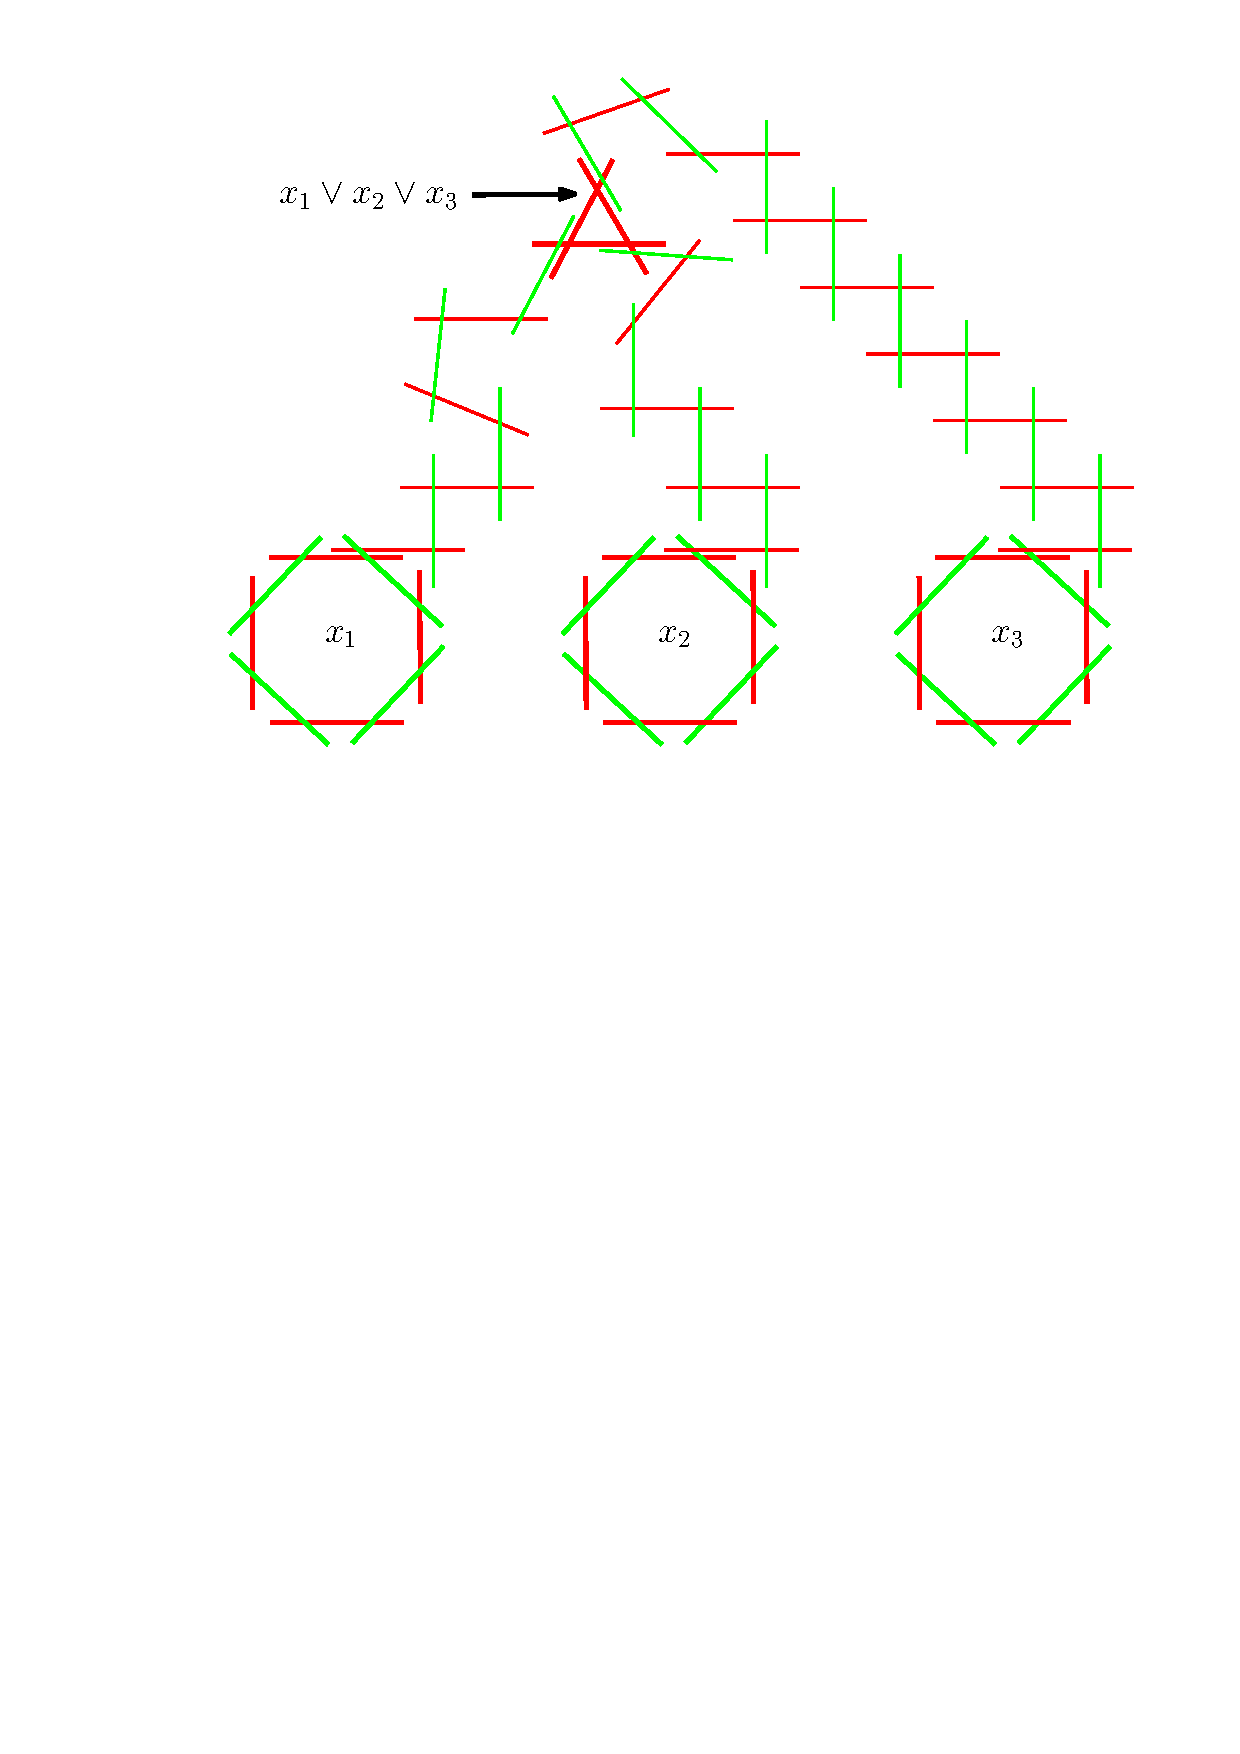
\includegraphics[width=.8\linewidth]{variable_clause_connection}
	\caption{Connection between the clause and variable gadgets, created by chains of an even number of segments.}
	\label{fig:gadget_connection}
\end{figure}

% Let $q$ be the number of clauses and $p$ be the number of distinct variables in $\phi$.
%
% \begin{lemma}
% 	\label{lem:optimal value}
% 	The construcetd Graph G has an optimal  value in terms of maximizing ink of $8q + 6mp + 9qt - (4q + 2p)\varepsilon$ if $\varepsilon$ is chosen sufficiently small.
% \end{lemma}
%
% \begin{proof}
% 	\soeren{i have an idea for this but i don't know if it would be out of scope, or if i might not even need this lemma. Also is our \maxsped defined as "Does this graph have a drawing with at least x amount of ink?" since thats what this bound is aiming at?"}
% \end{proof}
\soeren{it also still needs to be shown that this bound ensures that the two criterias from~\cite{b-sgh-15}, namely that at least one edge in the triangle is drawn and that the segment chains are alternatingly drawn and not drawn.}


	Let $\phi$ be a boolean formula and $\Pi$ be a planar embedding corresponding to that formula sucht that ($\phi$, $\Pi$) is an instance of \ppsat. Let $\Gamma$ be a drawing constructed from that instance in the previously described way. We will show that there is a valid truth assignement for $\phi$ if and only if $\Gamma$ admits a \maxsped with a value of at least $8q + 6mp + 3q (3t - 4\varepsilon)$ in terms of maximizing ink.
	~
	\begin{enumerate}
		\item[$\Rightarrow$:] Let $x$ be a variable and $c$ be a clause containing $x$. If $x$ is true draw all red edges in the associated variable gadget completely, which in turn means all green edges are drawn partially and vice versa for when $x$ is false. By drawing the green edges partially we enable the red edges in the segment chains to be drawn completely (if we shorten the stubs for one green edge in the variable gadget by $\varepsilon$). this also means we can draw the edges of the clause gadgets to which this segment chain is connected completely. Since $\phi$ has a satisfying variable assignement where exactly one variable per clause is true we have exactly one of these segment chains which allows exactly one edge per clause graph to be drawn completely. This results in every clause graph having the value $8 - 4\varepsilon$, every variable gadget having the value of $6m - 2\varepsilon$ and every segment chain having the value of $3t$. Let $q$ be the number of clauses and $p$ be the number of distinct variables in $\phi$. This results in 
		
		\soeren{is there a nice way to format this?}
		$(8 - 4\varepsilon)q + (6m - 2\varepsilon)p + 3t*3q = $
		$8q + 6mp + 9qt - (4q + 2p)\varepsilon$
		
		\item[$\Leftarrow$:]  Assume $\phi$ does not have a stisfying variable assignement. Then there must always exist a clause in which all three contained variables $x_1$, $x_2$ and $x_3$ are false. That however means that, by construction, there is a clause gadget where all the corresponding variable gadgets have all their green edges completely drawn. This adds at most the value of $2\varepsilon$. In order to get the maximal drawing, this propagates through the segment chains up to the clause gadget where it causes all three edges of that gadget to be not drawn. This in turn means that this specific gadget has only the value $6 - 6\varepsilon$. The total value of this drawing in terms of maximizing ink is therefore at least $2$ smaller than normal. If we would try to supplement the missing drawn edge of the clause gadget, we would need to switch up the alternation of drawing segments in the chains, which causes 2 consecutive segments to not be drawn. Since the last edge in the chain was dran before, it now can't be drawn and it therefore again results in a difference of at least $2$ in the complete drawing.
	\end{enumerate}


\soeren{TODO: argue equivalence (both direction)}

\end{proof}

\section{Two polynomial special cases}

%\begin{itemize}
%	\item dynamic programming
%	\item table entries $T_i(s)$ for $i = 1, \dots, \deg(s)$
%	\item $i$ corresponds to increasing stub lengths
%	\item stub lengths $l_i(s)$ for $i = 1, \dots, \deg(s)$ (not the pair of stubs)
%\end{itemize}

Section~\ref{sec:hardness} showed that \maxsped is generally \NP-hard for $k \ge 3$. In this section we consider the special case that the intersection graph of the $k$-plane input drawing is a tree or a cactus. Since every planar graph is representable as intersection graph of line segments~\cite{chalopin2009every}. we can also encounter every tree or cactus. In both cases we present polynomial-time dynamic programming algorithms. 

Let $ C = (V,E) $ be the intersection graph of the edge set $S$ in a given drawing $\Gamma$ of graph $ G $ as defined in Section~\ref{sec:preliminaries}. Let $ u \in V $ and $ \deg(u) = k $, then for the corresponding edge $ s(u) \in S $ there are $ k + 1 $ possible stub pairs including drawing the whole edge. We store the lengths of the possible stubs as node weights $ \ell_1(u), \dots, \ell_k(u) \in \mathbb{R}_+$ and assume that $ \ell_1(u),\dots,\ell_k(u) $ are sorted from shorter to longer stubs. We define  $ \ell_0(u) $ as the length of the whole edge $ s(u) $. 

%Computing the intersection graph requires to identify all the intersections in $ \Gamma $. Using a standard sweep line algorithm \cite{}\fabian{add citation} this requires $ O(|S|\log |S| + I) $ where $ I $ is the number of crossings. Building the graph then takes $ O(|S|) $ time. When computing the intersection we can compute the stub lengths and their order as well.
%
%\martin{time to build graph should be $O(S+I)$; but maybe this preparation work should go to preliminaries so that we can assume the intersection graph as input}
%\fabian{add to prelims}

\subsection{Trees}
\label{sec:tree}
Here we assume that the intersection graph $ C = (V,E) $ is a rooted tree of maximum degree $ k $. We give a bottom up dynamic programming algorithm for solving \maxsped on $ C $. For a vertex $ u \in V $ let $ p(u) $ denote the parent of $ u $ in $ C $ and let $ c(u) $ denote the set of its children. The ink values of the partial \maxsped solutions for the subtrees $T_u$ rooted at each vertex $ u \in V $ such that stub length $ \ell_i(u) $ is used for $s(u)$ are computed and stored as $ T_i(u) $.

\begin{figure}[tbp]
	\centering
	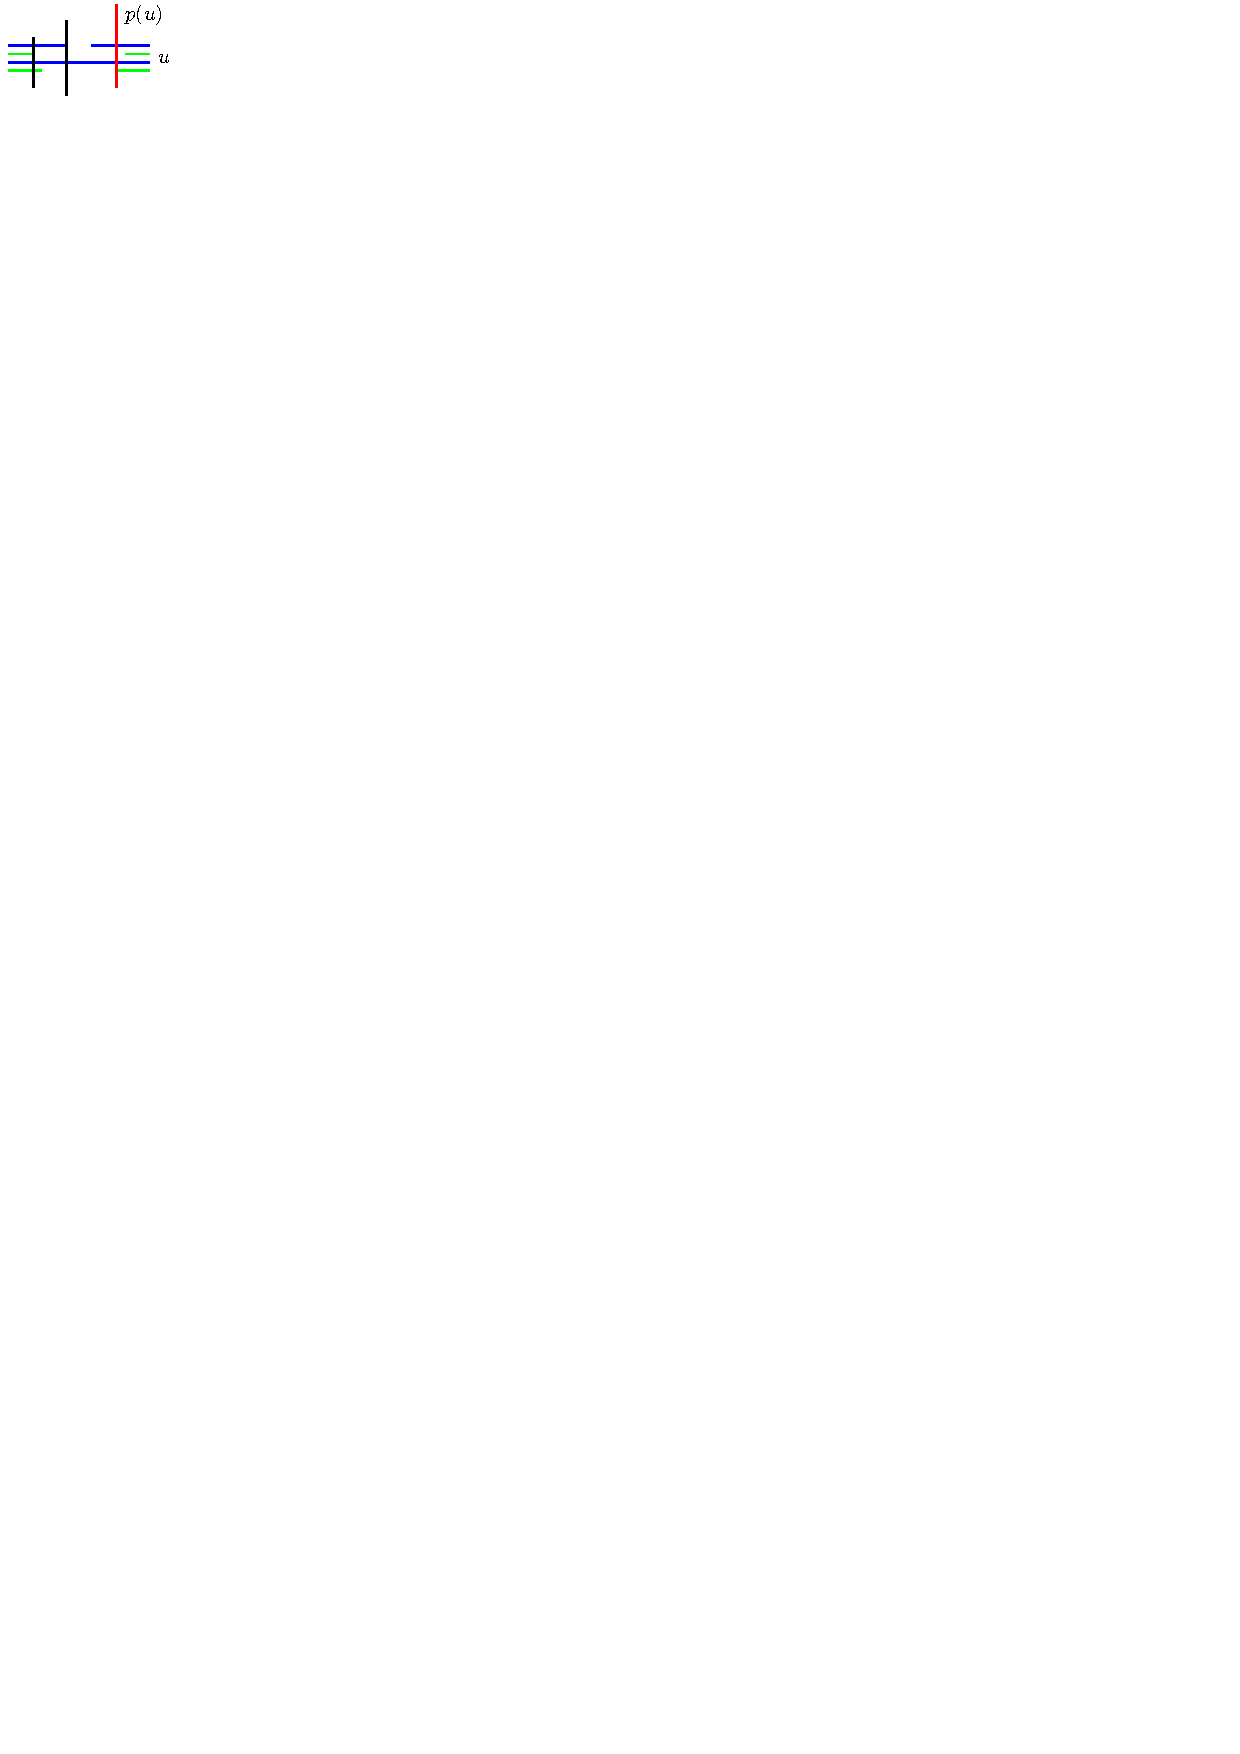
\includegraphics{two_solutions_needed}
	\caption{Consider $ u $, then only the blue and the green solution are relevant.}
	\label{fig:two_solutions}
\end{figure}

Since we know $ C $ is a tree every vertex $ u \in V $ with degree $ \delta $ has a parent $ p(u) \in V $. For this parent there exists one stub length $ \ell_j(p(u)) $ in the sequence of stub lengths $ \ell_0(p(u)),\dots,\ell_{\delta}(p(u)) $ such that drawing $ p(u) $ with these stubs does not intersect a completely drawn $ u $, while drawing $ p(u) $ with $ \ell_{j + 1}(p(u)) $, i.e. the next longer stub length, intersects $ \ell_0(u) $. We call the solution which would intersect the parent $ \sollong(u) $ and the one not intersecting the parent $ \solshort(u) $. See Figure~\ref{fig:two_solutions} for an illustration. More formally let $ j $ be the index such that stubs of length $ \ell_j(p(u)) $ do not intersect $ s(u) $, but $ \ell_{j +1}(p(u)) $ would, we set:
\begin{align*}
	\solshort(u) = \max\{T_1(u),\dots,T_j(u)\} \\
	\sollong(u) = \max\{T_0(u),\dots,T_{\delta}(u)\}
\end{align*}
It remains to define $ T_i(u) $ for a vertex $ u $ and stub length $ \ell_i(u) $:
\begin{align}
	\label{rec:tree}
	T_i(u) = \ell_i(u) + \sum_{v \in c(u)}
	\begin{cases}
		\solshort(v) & \text{if } s(u) \text{ with length } \ell_i \text{ intersects } s(v) \\
		\sollong(v) & \text{else}
	\end{cases}
\end{align}
Solving Recurrence~\ref{rec:tree} yields an optimal solution to the \maxsped problem on $ G $ with drawing $ \Gamma $ as the following lemma shows.

\begin{lemma}
	\label{lem:tree_correctness}	
	Let $ G $ be a simple graph and $ \Gamma $ a straight-line drawing of $ G $. If the intersection graph $ C = (V,E) $ of $ G $ is a tree with root $ r \in V $ and maximum degree $ k $, then $ \sollong(r) = \max \{T_i(r) \mid 0 \leq i \leq k \} $ is an optimal solution to the \maxsped problem on $ G $ with drawing $ \Gamma $.
\end{lemma}
\begin{proof}
	Let $ G $, $ \Gamma $ and $ C = (V,E) $ as above and $ u \in V $ a leaf of $ C $. Since $ c(u) $ is empty we simply get $ \solshort(u) = T_0(u) = \ell_1(u) $ and $ \sollong(u) = T_1(u) = \max\{\ell_0(u), \ell_1(u)\} $. Now let $ u \in V $ with degree $ \delta $ be an inner vertex. The values $ \solshort(v) $ and $ \sollong(v) $ are computed for all $ v \in c(u) $. $ T_i(u) $ for one $ 0 \leq i \leq \delta $ is then the sum of the maximum stubs we can draw among the children plus the stub length $ \ell_i(u) $ itself, which are just the values we are interested in. Setting then $ \sollong(u) $ and $ \solshort(u) $ as above gives the two necessary values for $ p(u) $.
	
%	and $ t = \sollong(r) $ is the maximum value for some $ T_i(r) $'s and $ r $ the root. Now let $ t' $ be the value of a solution to the \maxsped problem on $ G $ with drawing $ \Gamma $ and $ t' > t $. This solution has to be the sum of a set of stub lengths for each edge in $ G $ such that no two stubs intersect by definition. Further we know the stubs can be categorized into two sets relative to their parent. Recurrence~\ref{rec:tree} builds just the maximum over the $ \solshort(v) $ and $ \sollong(v) $ values for all $ v \in c(u) $, such that no two stubs intersect. Hence if $ t $ was not optimal we would need to find at least a third stub length for at least one child $ v \in c(u) $ which was neither equal to $ \sollong(v) $ nor $ \solshort(v) $.
\end{proof}

\begin{figure}
	\centering
	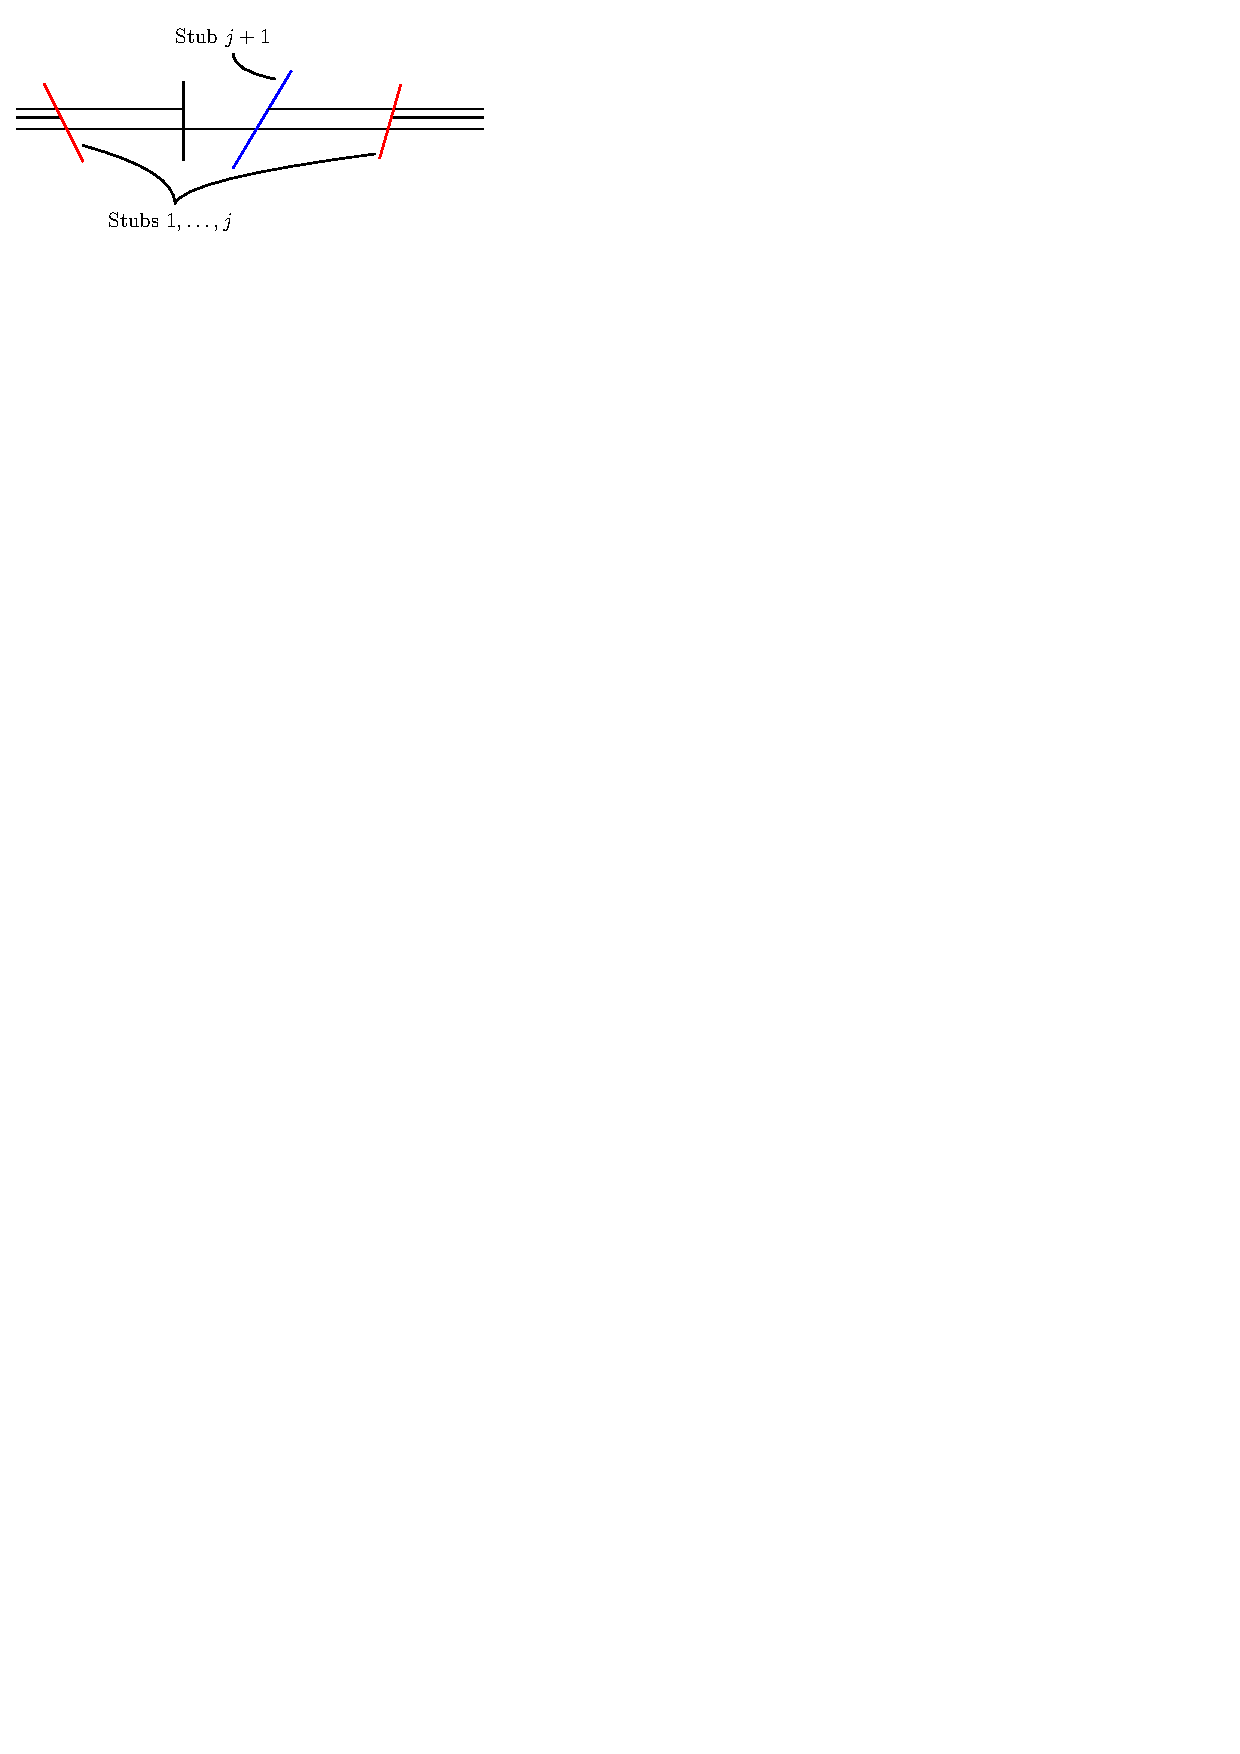
\includegraphics{speedup}
	\caption{The situation in Lemma~\ref{lem:compute_vertex}.}
	\label{fig:speedup}
\end{figure}
Solving Recurrence~\ref{rec:tree} straight forward would yield an algorithm running in $ O(mk^2) $. Using the order on the stub lengths though we can improve this to $ O(mk) $ by solving $ T_i(u) $ in linear time for one $ u \in V $.

\begin{lemma}
	\label{lem:compute_vertex}
	Let $ C = (V,E) $ be a tree with maximum degree $ k $ and vertex weights $ \ell_0,\dots,\ell_{\delta} $ for every $ u \in V $ with degree $ \delta $. We can compute $ \solshort(u) $ and $ \sollong(u) $ in $ O(\delta) $ time and space, if the values $ \sollong(v) $ and $ \solshort(v) $ are computed for all children $ v \in c(u) $.
\end{lemma}
\begin{proof}
	 Let $ u \in V $ be a vertex with degree $ \delta < k $ for which we have computed $ \sollong $ and $ \solshort $ for every of its children. The crucial part is that $ T_i(u) $ can be built iteratively by going through the list of stub lengths for $ u $ in ascending order. First we compute $ T_1(u) $, this is the solution for $ u $ in which we are able to draw the children with any of their stub lengths. This means we need to build the sum of $ \ell_1(u) $ and the $ \sollong(v) $ for every $ v \in c(u) $ which runs in $ O(\delta) $. The same can be done for $ T_0(u) $, but taking all the $ \solshort(v) $ values for the children $ v \in c(u) $. Assume we computed $ T_j(u) $ for all stub lengths $ \ell_i(u) $ with $ i \leq j $. Now we want to compute $ T_{j+1}(u) $ (see Figure~\ref{fig:speedup}). By drawing $ s(u) $ with stub length $ \ell_{j +1} $ we make it a bit longer since we consider the $ \ell_i(u) $ in ascending order. Hence by doing so we now potentially intersect the corresponding edge of the $ j $-th child $ v_j \in c(u) $. Since $ s(v_j) $ is the only segment affected by drawing $ u $ with stub length $ \ell_{j + 1} $ instead of $ \ell_j $ we can compute $ T_{j+1}(u) $ in $O(1)$ time by simply subtracting $ \sollong(v) $ and adding $ \solshort(v) $.
	
	Finally we need to compute $ \solshort(u) $ and $ \sollong(u) $, but this are just two maximizations over at most $ \delta + 1 $ values at most. This can be done in $ O(\delta) $ by simply sweeping over the values.
\end{proof}

\begin{theorem}
	\label{thm:tree}
	Let $ G $ be a simple graph with $m$ edges and $ \Gamma $ a straight-line drawing of $ G $. If the intersection graph $ C = (V,E) $ of $ G $ is a tree with maximum degree $ k \in \mathbb{N} $ the \maxsped problem can be solved in $ O(mk + m \log m)) $ time and space.
\end{theorem}
\begin{proof}
	Since $ C $ is known to be a tree, and hence $ |E| = O(m) $, we can compute the intersection graph and the stub lengths in $ O(m\log m) $ time and space.
	
	To solve the \maxsped problem on $ G $ we need to compute $ \max \{T_i(r) \mid 0 \leq i \leq k \} $ for the root $ r \in V $ of $ C $ by Lemma~\ref{lem:tree_correctness}. Doing this bottom up requires one pass through $ C $ hence by applying Lemma~\ref{lem:compute_vertex} we need $ O(mk) $ time to compute all $ T_i(u) $ for all $ u \in V $. For every vertex we only need to compute $ O(k) $ values and store two of them, namely $ \sollong(u) $ and $ \solshort(u) $, so we do not need more than $ O(mk) $ memory. Adding the bounds yields the desired runtime of $ O(mk + m \log m)) $.
	
	Retrieving the actual stub length for each edge in $ G $ needed to produce the SPED can be done by backtracking the subsolutions which requires at most $ O(mk) $ time.
\end{proof}

\martin{the figures can still be improved in style and size; maybe merge into one, use nicer colors, draw just one segment and not multiple shifted ones etc}

%\begin{itemize}
%	\item segment $s$ with $d$ children $u_1, \dots, u_{d}$ and parent $p(s) = p$.
%	\item Assume children are sorted by their intersection points on $s$, i.e., $u_1$ produces stub length $l_1$ etc.
%	\item for stub length relating to parent use offset from next longer stub length
%\end{itemize}

\subsection{Cacti}
\label{sec:cactus}
In this section we restrict $ C = (V,E) $ to be a cactus graph, i.e. a simple graph in which no edge $ e \in E $ is part of more than one cycle. For a cactus graph $ C $ the \emph{block-cut tree} is the tree $ \mathcal T = (\mathcal V, \mathcal E) $where $ \mathcal V $ contains a vertex for every cycle and \emph{cut vertex} in $ C $. We call a vertex $ u \in \mathcal V $ a \emph{block vertex} if it represents a cycle and \emph{articulation vertex} else. For a block vertex $ u \in \mathcal V $ representing an induced cycle with vertices $ V_c \subseteq V $ we define $ \textit{cycle}(u) = V_c$. For an articulation vertex $ u \in \mathcal V $ representing the cut vertex $ v \in V $ we define $ A(u) = v $. There is an edge $ uv \in \mathcal E $ between a block vertex $ u $ and articulation vertex $ v $ whenever $ v \in \textit{cycle}(u) $ and an edge $ uv \in \mathcal E $ between two articulation vertices whenever $ A(u)A(v) $ was an edge in $ E $.

Let $ C = (V,E) $ be a cactus graph and moreover the intersection graph of a graph $ G $ and straight-line drawing $ \Gamma $. Additionally let $ \mathcal T = (\mathcal V, \mathcal E) $ be the block-cut tree of $ C $ we define for each vertex $ u \in \mathcal V $ two values $ a,b \in \mathbb{R}_+ $, w.l.o.g $ a \leq b $. If $ u $ is an articulation vertex this are exactly the positions where the cycle represented by $ p(u) $ intersects $ s(A(u)) $ in $ \Gamma $. If $ u $ is a block vertex $ a,b $ are the points where the by $ \textit{cycle}(u) $ represented edges intersect $ s(A(p(u))) $. Similar to Section~\ref{sec:tree} we define three values for every vertex $ u \in \mathcal V $ with degree $ \delta $:
\begin{align*}
	\solshort(u) &= \max\{T_0(u),\dots,T_\delta(u)\}\\
	\solmid(u) &= \max\{T_1(u),\dots,T_{a}(u)\}\\
	\sollong(u) &= \max\{T_1(u),\dots,T_{b}(u)\}\\
\end{align*}

For an articulation vertex $ u \in \mathcal V $:
\begin{align}
\label{rec:cactus_articulation}
T_i(u) = \ell_i(A(u)) + \sum_{v \in c(u)}
\begin{cases}
\solshort(v) & \text{if } \ell_i(A(u)) \leq a \\
\solmid(v) & \text{if } a < \ell_i(A(u)) \leq b \\
\sollong(v) & \text{else}
\end{cases}
\end{align}

\begin{lemma}
	\label{lem:cactus_correctness}	
	Let $ G $ be a simple graph and $ \Gamma $ a straight-line drawing of $ G $. If the intersection graph $ C = (V,E) $ of $ G $ is a cactus with root $ r \in V $ and maximum degree $ k $, then $ \sollong(r) = \max \{T_i(r) \mid 0 \leq i \leq k \} $ is an optimal solution to the \maxsped problem on $ G $ with drawing $ \Gamma $.
\end{lemma}
\begin{proof}	
	Let $ G $, $ \Gamma $,  $ C = (V,E) $ and $ \mathcal T = (\mathcal V,\mathcal E) $ as above and $ u \in \mathcal V $ a leaf of $ \mathcal T$. Then either $ u $ is an articulation vertex and to be treated as in Lemma~\ref{lem:compute_vertex} or a cycle. In the latter case we find the optimal solution to the \maxsped problem on $ C[\textit{cycle}(u)] $ with the algorithm from Bruckdorfer et al. \cite{bcgkmn-pped-17}. Using the above described method we derive $ \solshort(u) $, $ \solmid(u) $ and $ \sollong(u) $, this are exactly the optimal values depending on how the cycle interacts with the articulation vertex $ p(u) $.

	Now let $ u \in V $ with degree $ \delta $ be an inner vertex of $ \mathcal T $. The values $ \solshort(v) $, $ \solmid(v) $ and $ \sollong(v) $ are computed for all $ v \in c(u) $. Again first let $ u $ be an articulation vertex, then the maximum for stub $ \ell_i(A(u)) $ is said value plus the sum of the compatible children, which is just Recurrence~\ref{rec:cactus_block}. Now let $ u $ be a block vertex. We have to cut open the cycle it represents (compare \cite{bcgkmn-pped-17}). We do this at $ p = A(p(u)) $. The resulting graph is a path over the vertices in $ \textit{cycle}(u) $ with attached articulation vertices. This is especially a tree and we use the aglorithm from Section~\ref{sec:tree}, maximizing over three values of the articulation vertices though,  to compute the $ T_i(u) $.
\end{proof}

\begin{lemma}
	\label{lem:compute_articulation}
	Let $ \mathcal T = (\mathcal V,\mathcal E) $ be a cactus with maximum degree $ k $ and vertex weights $ \ell_0,\dots,\ell_{\delta} $ for every articulation vertex $ u \in \mathcal V $ with degree $ \delta $. We can compute $ \solshort(u) $, $ \solmid(u) $ and $ \sollong(u) $ in $ O(\delta) $ time and space, if the values $ \sollong(v) $, $ \solmid(v) $ and $ \solshort(v) $ are computed for all children $ v \in c(u) $.
\end{lemma}
\begin{proof}
	Follows from Lemma~\ref{lem:compute_vertex}, since an articulation vertex has at most $ \delta $ many children in $ \mathcal{T} $, one for each cycle it is part of in $ C $ and one for every other articulation vertex it was already connected to in $ C $. 
\end{proof}

\begin{lemma}
	\label{lem:compute_block}
	Let $ \mathcal T = (\mathcal V,\mathcal E) $ be a cactus with maximum degree $ k $ and vertex weights $ \ell_0,\dots,\ell_{\delta} $ for every block vertex $ u \in \mathcal V $ with degree $ \delta $. We can compute $ \solshort(u) $, $ \solmid(u) $ and $ \sollong(u) $ in $ O(n\delta) $ time and space, if the values $ \sollong(v) $, $ \solmid(v) $ and $ \solshort(v) $ are computed for all children $ v \in c(u) $.
\end{lemma}
\begin{proof}
	Let $ G $, $ \Gamma $,  $ C = (V,E) $ and $ \mathcal T = (\mathcal V,\mathcal E) $ as above and $ u \in \mathcal V $ a block vertex with degree $ \delta $. Computing the value for the cycle itself $ \textit{cycle}(u) $ takes $ O(n) $ time by Bruckdorfer et al. Now at every vertex $ v \in \textit{cycle}(u) $ there might be a set of up to $ \delta $ many children, which are all articulation points. Their values are already known and maximization over them can hence be done in $ O(\delta) $ time by the same argument as in Lemma~\ref{lem:compute_vertex}. Following we need $ O(n\delta) $ to compute the three values $ \solshort(u) $, $ \solmid(u) $ and $ \sollong(u) $.
\end{proof}

\begin{theorem}
	Let $ G $ be a simple graph with $m$ edges and $ \Gamma $ a straight-line drawing of $ G $. If the intersection graph $ C = (V,E) $ of $ G $ is a cactus with maximum degree $ k \in \mathbb{N} $ the \maxsped problem can be solved in $ O(mk^2 + m \log m)) $ time and space.
\end{theorem}
\begin{proof}
	Follows as in Theorem~\ref{thm:tree} by maximizing over the tree using Lemma~\ref{lem:cactus_correctness} and Recurrence~\ref{rec:cactus_articulation}. Then the running time follows from constructing the intersection graph and the block-cut tree as well as Lemma~\ref{lem:compute_articulation} and~\ref{lem:compute_block}.
\end{proof}




\section{Conclusion}


\bibliography{paper}

\end{document}
